\documentclass[11pt, oneside]{article}
\usepackage{titling, geometry, hyperref, fancyhdr, algorithm, enumitem}
\usepackage{amsmath, amssymb, amsthm}              % mathematical packages
\usepackage{graphicx, subcaption, wrapfig}         % images
\usepackage{textcomp, CJKutf8}                     % misc. text formatting
\usepackage{tikz, pgfplots, tikz-network}          % plots and graphs
\usepackage[noend]{algpseudocode}                  % algorithm psuedocode
\usepackage[cache=true]{minted}                    % source code
\usepackage[style=numeric, sorting=none]{biblatex} % bibliography
\geometry{a4paper}

\hypersetup{
  colorlinks=true,
  urlcolor=cyan
}

% https://tex.stackexchange.com/questions/343494/minted-red-box-around-greek-characters
\makeatletter
\AtBeginEnvironment{minted}{\dontdofcolorbox}
\def\dontdofcolorbox{\renewcommand\fcolorbox[4][]{##4}}
\makeatother

\newcommand{\emphasis}[1]{\textbf{\textit{#1}}}
\graphicspath{{./images/}}
\addbibresource{ref.bib}

\title{Physics of Railgun}
\author{Stephen Huan}
\date{July 2, 2020}

\newcommand{\df}{\ensuremath{\text{ d}}}

\begin{document}
\maketitle

\section{Introduction}

\begin{CJK}{UTF8}{maru} 
The anime \href{https://myanimelist.net/anime/6213/Toaru_Kagaku_no_Railgun}
{とある科学の超電磁砲} 
(romanized as \textit{Toaru Kagaku no Choudenjihou}, 
translated as \textit{A Certain Scientific Railgun}) has a main character,
Mikoto Misaka who is able to use electromagnetic fields to accelerate metal 
objects to high velocity. However, there are those among us who doubt
the physical accuracy of such a power.
\end{CJK}

\begin{figure}[h!]
  \centering
  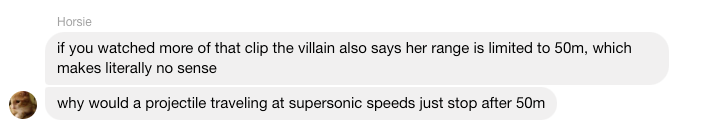
\includegraphics[scale=0.6]{message}
  \caption{A disbeliever}
\end{figure}

Thus, we shall begin to analyze her powers with physics.

\section{Determining Parameters}

First, Misaka usually shoots coins. We will assume the coin she shoots 
is roughly equivalent to a modern day Japanese 100 yen coin, 
though the selection of the coin will not vary the end result too much.

\begin{wrapfigure}{r}{0.25\textwidth}
  \vspace{-20pt}
  \centering
  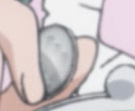
\includegraphics[scale=0.8]{100yen}
  \caption{It is hard to see, but this appears to be a 100 yen coin. (Episode 20, 11:05)}
  \vspace{-40pt}
\end{wrapfigure}

A \href{https://en.wikipedia.org/wiki/Japanese_yen}{100 yen coin}
has a mass of 4.8g, a diameter of 22.6mm, and a 
thickness or height of 1.7mm. Second, we need to calculate the effect of air 
resistance on the coin, which is the primary force slowing the motion of the 
coin as it travels through the air. In order to calculate drag from air 
resistance, we will need to know \( \rho \), the air density, 
\( A \), the effective area, and \( C_d \), the coefficient of drag
which is a function of the shape of the object as it travels through the air.
The \href{https://en.wikipedia.org/wiki/Density_of_air}{density of air}
at \( 20^{\circ} \) C is 1.2041 kg/\( \text{m}^3 \).

\newpage

\begin{figure}[t!]
  \centering
  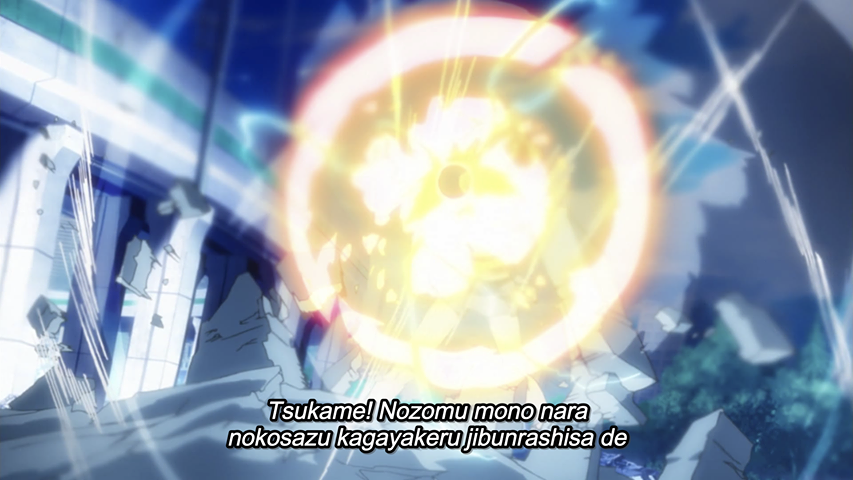
\includegraphics[scale=0.45]{shot}
  \caption{Misaka shooting a coin in the intro (Episode 1, 2:46)}
\end{figure}

From the image, the face of the coin is clearly visible and is upright,
meaning she shoots it such that the face is traveling forward. 
The \href{https://www.engineersedge.com/fluid_flow/circular_flat_disk_drag_coefficient_14035.htm#:~:text=The%20drag%20coefficient%20(non%2Ddimensional,velocity%20pressure%20and%20frontal%20area.&text=Coefficients%20are%20given%20for%20a,for%20cars%2C%20airships%20and%20struts.}
{coefficient of drag} for a flat disk is 1.12.
The area of the coin perpendicular to the direction of motion 
is the area of its face, or \( \pi r^2 \).
Thus, \( A = \pi r^2 = \pi (\frac{22.6 \text{ mm}}{2})^2 
= 4.01 \cdot 10^{-4} \text{ m}^2 \). 

Next, Misaka fires the coins at a velocity of 1030 m/s.
\begin{figure}[h!]
  \centering
  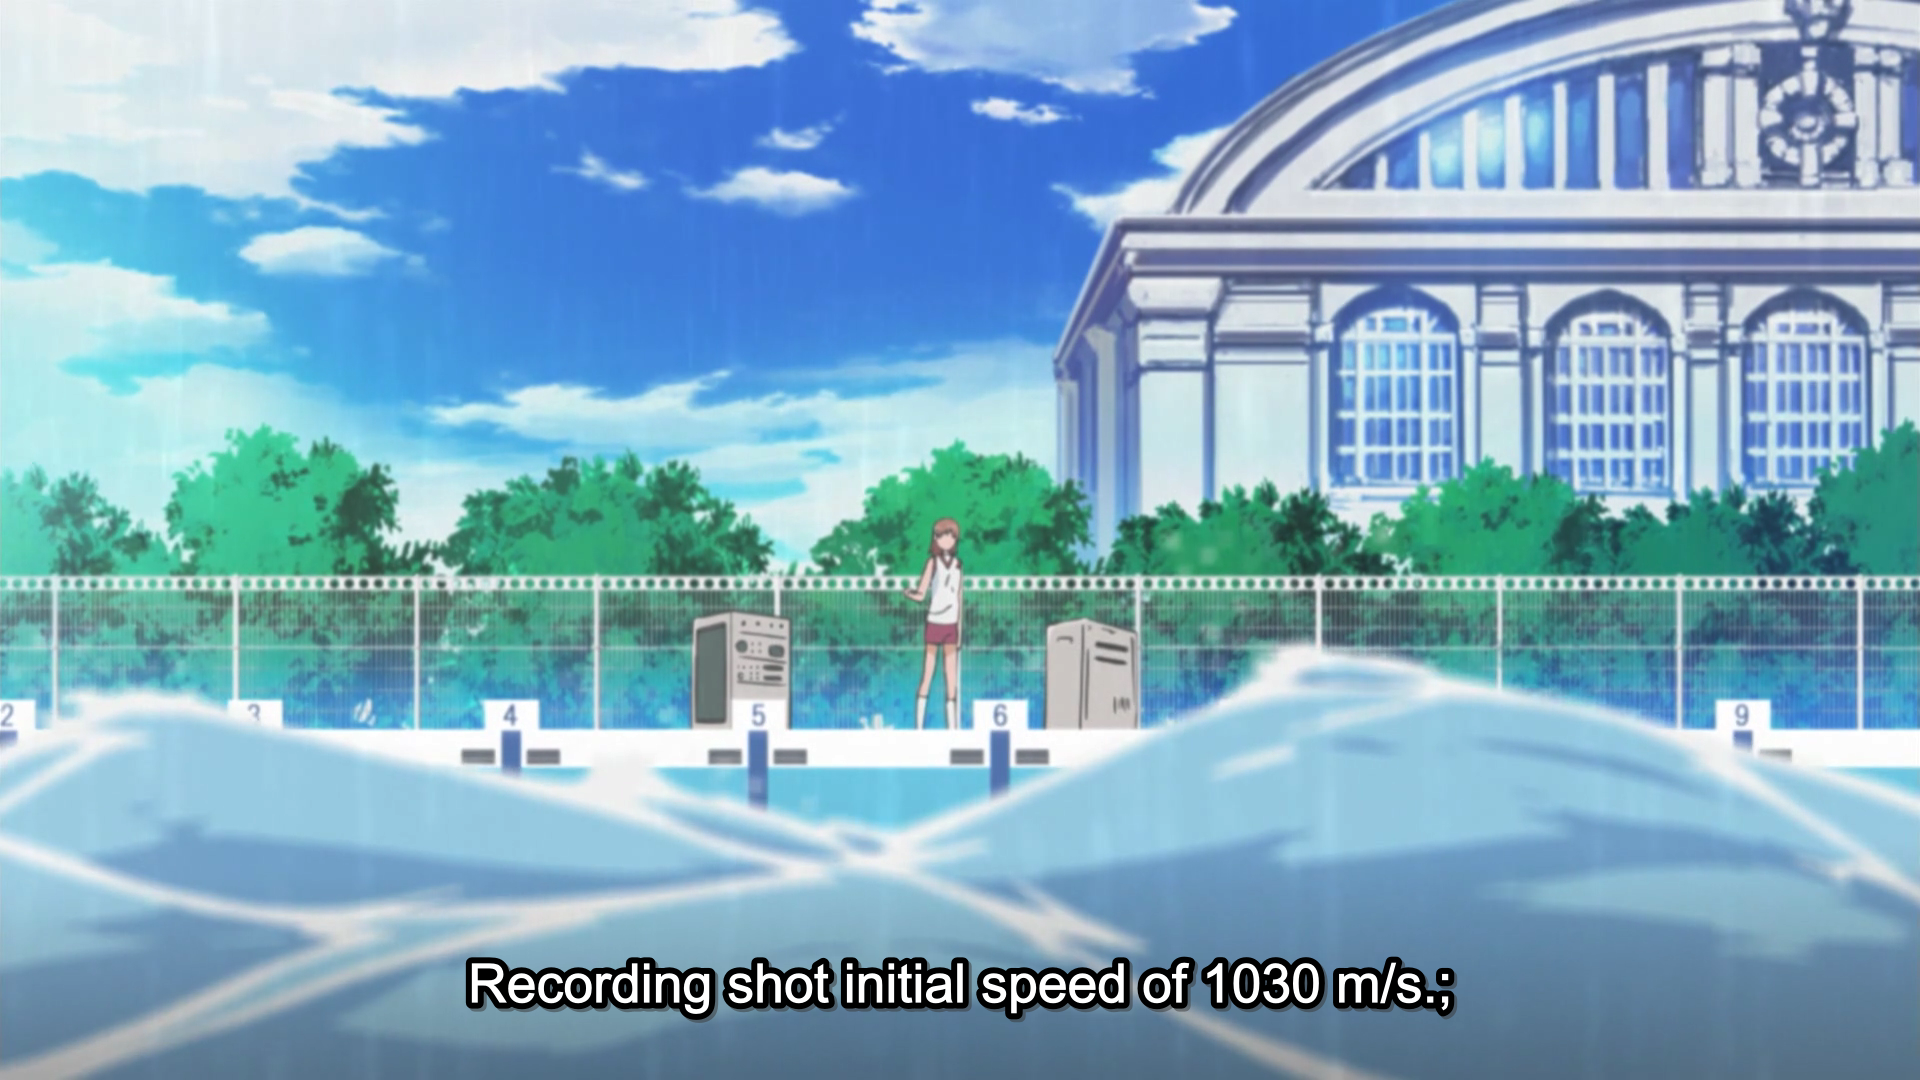
\includegraphics[scale=0.2]{speed}
  \caption{Measured speed of the coin (Episode 1, 7:53)}
\end{figure}

In order to calculate how long it takes for the coin to hit the ground,
we will need to know Misaka's height.
She is \href{https://toarumajutsunoindex.fandom.com/wiki/Misaka_Mikoto}
{161 cm} tall, and we can assume her arms are roughly 3/4 of that height,
putting the starting height of the coin at 120 cm.

Lastly, we might want to calculate the ballistics for a bullet rather than 
a coin, which might be interesting. Using the \href{https://www.hornady.com/bullets/eld-match}
{Hornady ELD (extreme low drag)} bullets, 
we \href{https://arxiv.org/pdf/1608.06500.pdf}{find} that
it has a weight of 13.5g, a diameter of 7.62mm, and a \( C_d \) of 0.242.
The area is then the area of the face, or \( \pi r^2 \) again.
\( \pi (\frac{7.62 \text{ mm}}{2})^2 = 4.56 \cdot 10^{-5} \) m\(^2\).

To summarize:
\begin{table}[h]
    \centering
    \begin{tabular}{| c | c | c | c |}
        \hline
        Description & Symbol & Value & Unit \\
        \hline
        Mass of coin & \( m \) & 4.8 & g \\
        Diameter of coin & \( d \) & 22.6 & mm \\
        Air density & \( \rho \) & 1.2041 & kg/m\(^3\) \\
        Area & \( A \) & \( 4.01 \cdot 10^{-4} \) & m\(^2\) \\
        Coefficient of drag & \( C_d \) & 1.12 & n/a \\
        Initial velocity & \( v_0 \) & 1030 & m/s \\ 
        Time elapsed & \( t \) & n/a & s \\
        Height & \( h \) & 120 & cm \\
        Gravity of Earth & \( g \) & 9.81 & m/s\(^2\) \\
        Mass of bullet & \( m \) & 13.5 & g \\
        Area of bullet & \( A \) & \( 4.56 \cdot 10^{-5} \) & m\(^2\) \\
        Coefficient of drag & \( C_d \) & 0.242 & n/a \\
        \hline
    \end{tabular}
    \caption{List of variables}
\end{table}

\section{Problem Statement}
Because we are AP physics students, here is a proper problem statement:

Mikoto Misaka, the ``railgun'', fires a 100 yen coin at 1030 m/s 
at her latest enemy, who is standing at a distance of 50m away.
However, the coin experiences drag from air resistance 
as it flies through the air with its face towards the enemy.
\begin{enumerate}[label=\alph*.]
    \item Find the velocity of the coin as a function of time.
    \item Find the horizontal distance of the coin from Misaka as a function of time.
    \item How far does the coin travel? Does she hit her enemy?
\end{enumerate}

\section{Solution}

The \href{https://en.wikipedia.org/wiki/Drag_equation}{Drag equation}
gives the force of drag as \( F_d = \frac{1}{2} \rho v^2 A C_d \).
For clarity, let \( k = \frac{1}{2} \rho A C_d \).
The force is also negative since it opposes the velocity of the coin.
\begin{align*}
    F_d &= -kv^2 \\
    a &= \frac{F}{m} = \frac{\df v}{\df t} \\
    \df v &= \frac{F}{m} \df t \\
          &= -\frac{k}{m}v^2 \df t \\
    \int^{v_f}_{v_0} \frac{1}{v^2} \df v &= -\int^t_0 \frac{k}{m} \df t \\
    [ -v^{-1} ]^{v_f}_{v_0} &= -\frac{k}{m} t \\
    \frac{1}{v_0} - \frac{1}{v_f} &= -\frac{k}{m} t \\
    v_f &= \frac{1}{\frac{1}{v_0} + \frac{k}{m} t} = \boxed{\frac{v_0}{1 + \frac{v_0 k}{m} t}} \text{ a.}
\end{align*}
Essentially, the velocity starts at \( v_0 \) and decreases as time grows bigger
like the function 1/x. To find position, simply integrate over velocity.
Let \( c = \frac{v_0 k}{m} = \frac{v_0 \rho A C_d}{2m} \).
\begin{align*}
    x &= \int^t_0 v(t) \df t \\
      &= \int^t_0 \frac{v_0}{1 + ct} \df t \\
      &= [\frac{v_0}{c} \ln (1 + ct)]^t_0 \\
      &= \boxed{\frac{v_0}{c} \ln(1 + ct)} \text{ b.}
\end{align*}

Lastly, to find the distance traveled we just need to calculate the 
time it takes before the coin hits the ground
(where we then assume it stops moving horizontally).
\begin{align*}
    h &= \frac{1}{2} gt^2 \\
    t &= \sqrt{\frac{2h}{g}} = 0.5 \text{ s} 
\end{align*}

Evaluating \( x(t) \) at \( t = 0.5 \):
First, \( c = 58.0 \) s\(^{-1}\), thus \( x(t) = \) \fbox{60.4m}. \newline

\section{Problem 2}
Suppose Misaka is tired of using coins, and upgrades her ammunition to 
the bullets described above. Assuming the coin reaches terminal velocity
from the railgun launch, how far does the bullet travel?

\section{Solution}

The acceleration of a \href{https://en.wikipedia.org/wiki/Railgun}{railgun} 
is given by 
\[ a = \frac{L' I^2}{2m} \] 
where \( L' \) is the inductance per meter, and \( I \) is the current.

The \href{https://en.wikipedia.org/wiki/Terminal_velocity}{terminal velocity}
can be derived from the drag equation given earlier, and is 
\[ v_t = \sqrt{\frac{2ma}{\rho A C_d}} \]

Combining the two equations yields the terminal velocity for a railgun:
\[ v_t = \sqrt{\frac{2ma}{\rho A C_d}} 
       = \sqrt{\frac{2m\frac{L' I^2}{2m}}{\rho A C_d}} 
       = \sqrt{\frac{L' I^2}{\rho A C_d}} \]

Squaring both sides, 
\[ L' I^2 =  {v_t}^2 \rho A C_d \]

Evaluating for the disk \( A \) and \( C_d \) and \( v_0 \) for \( v_t \)
one obtains 574 \(  H \cdot \) A\(^2\). 
Finding \( L' I^2 \) for a 
\href{https://apps.dtic.mil/dtic/tr/fulltext/u2/a253366.pdf}{military railgun},
\( 79.0 \cdot 10^4 \), or about 138x more powerful which is reasonable
considering the substantially smaller payload.

Finding the launch velocity for a bullet with the same terminal velocity 
equation, but with the bullet \( A \) and \( C_d \) yields a initial velocity
of 6,570 m/s. Finally, \( c \) is 3.23 s\(^{-1}\) and
the distance traveled is 1950m, or about two kilometers. 
This is an absurd 33x farther distance than the coin, 
and intuitively a bullet is a much more aerodynamic shape.

\section{Conclusion}

Railgun physics is absolutely correct; Mikoto Misaka best girl. \\

\printbibliography
\end{document}
